\documentclass[11pt]{article}
\usepackage[textwidth=18.0cm, textheight=23.0cm, top=2.0cm]{geometry}
\usepackage{pst-all}
\usepackage{amssymb}
\usepackage{tikz}
\usepackage{underscore}\begin{document}
\pagestyle{empty}


ClassName: \underline{\textbf{Class_03.2bp-39}}
\par
BinSize: \underline{\textbf{40 × 40}}
\par
ReduceSize: \underline{\textbf{40 × 40}}
\par
TypeNum: \underline{\textbf{79}}
\par
Num: \underline{\textbf{80}}
\par
OutS: \underline{\textbf{28800}}
\par
InS: \underline{\textbf{25943}}
\par
Rate: \underline{\textbf{0.901}}
\par
UB: \underline{\textbf{18}}
\par
LB0: \underline{\textbf{18}}
\par
LB: \underline{\textbf{18}}
\par
LBWithCut: \underline{\textbf{18}}
\par
NodeCut: \underline{\textbf{0}}
\par
ExtendedNodeCnt: \underline{\textbf{1}}
\par
GenNodeCnt: \underline{\textbf{1}}
\par
PrimalNode: \underline{\textbf{0}}
\par
ColumnCount: \underline{\textbf{18}}
\par
TotalCutCount: \underline{\textbf{0}}
\par
RootCutCount: \underline{\textbf{0}}
\par
LPSolverCnt: \underline{\textbf{1}}
\par
PricingSolverCnt: \underline{\textbf{0}}
\par
BranchAndBoundNum: \underline{\textbf{1}}
\par
isOpt: \underline{\textbf{true}}
\par
TimeOnInitSolution: \underline{\textbf{600.000 s}}
\par
TimeOnPrimal: \underline{\textbf{0.000 s}}
\par
TimeOnPricing: \underline{\textbf{0.000 s}}
\par
TimeOnRmp: \underline{\textbf{0.078 s}}
\par
TotalTime: \underline{\textbf{600.343 s}}
\par
\newpage


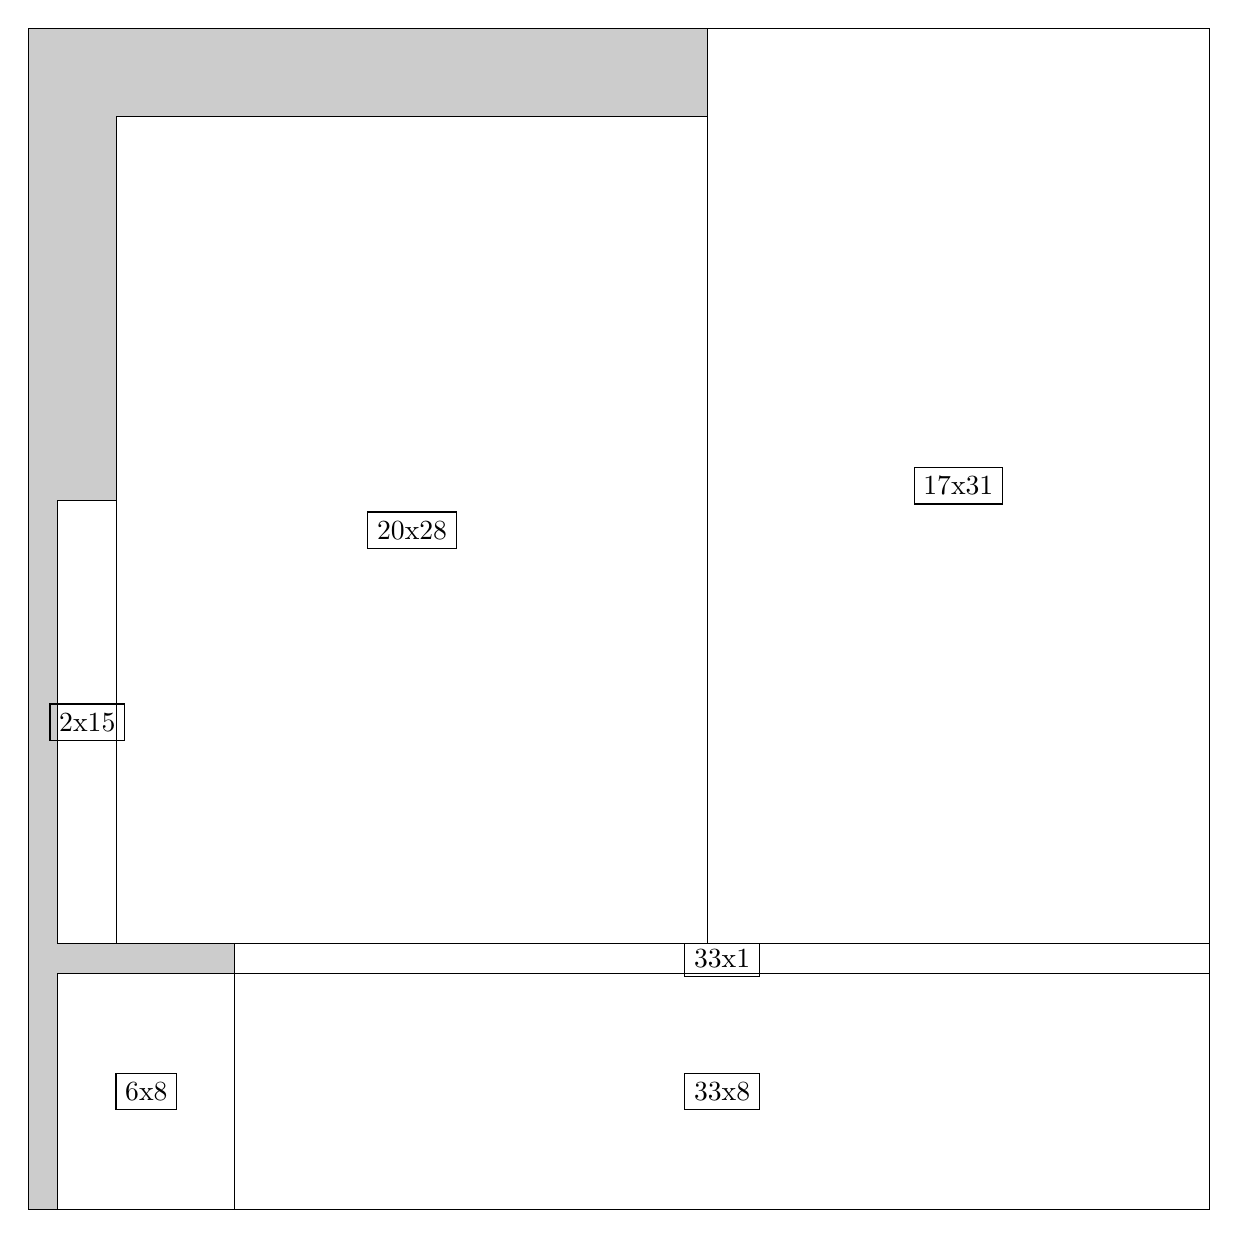
\begin{tikzpicture}[shorten >=1pt,scale=1.0,every node/.style={scale=1.0},->]
\tikzstyle{vertex}=[circle,fill=black!25,minimum size=14pt,inner sep=0pt]
\filldraw[fill=gray!40!white, draw=black] (0,0) rectangle (15.0,15.0);
\foreach \name/\x/\y/\w/\h in {33x8/2.625/0.0/12.375/3.0,33x1/2.625/3.0/12.375/0.375,6x8/0.375/0.0/2.25/3.0,17x31/8.625/3.375/6.375/11.625,20x28/1.125/3.375/7.5/10.5,2x15/0.375/3.375/0.75/5.625}
\filldraw[fill=white!40!white, draw=black] (\x,\y) rectangle node[draw] (\name) {\name} ++(\w,\h);
\end{tikzpicture}


w =33 , h =8 , x =7 , y =0 , v =264
\par
w =33 , h =1 , x =7 , y =8 , v =33
\par
w =6 , h =8 , x =1 , y =0 , v =48
\par
w =17 , h =31 , x =23 , y =9 , v =527
\par
w =20 , h =28 , x =3 , y =9 , v =560
\par
w =2 , h =15 , x =1 , y =9 , v =30
\par
\newpage


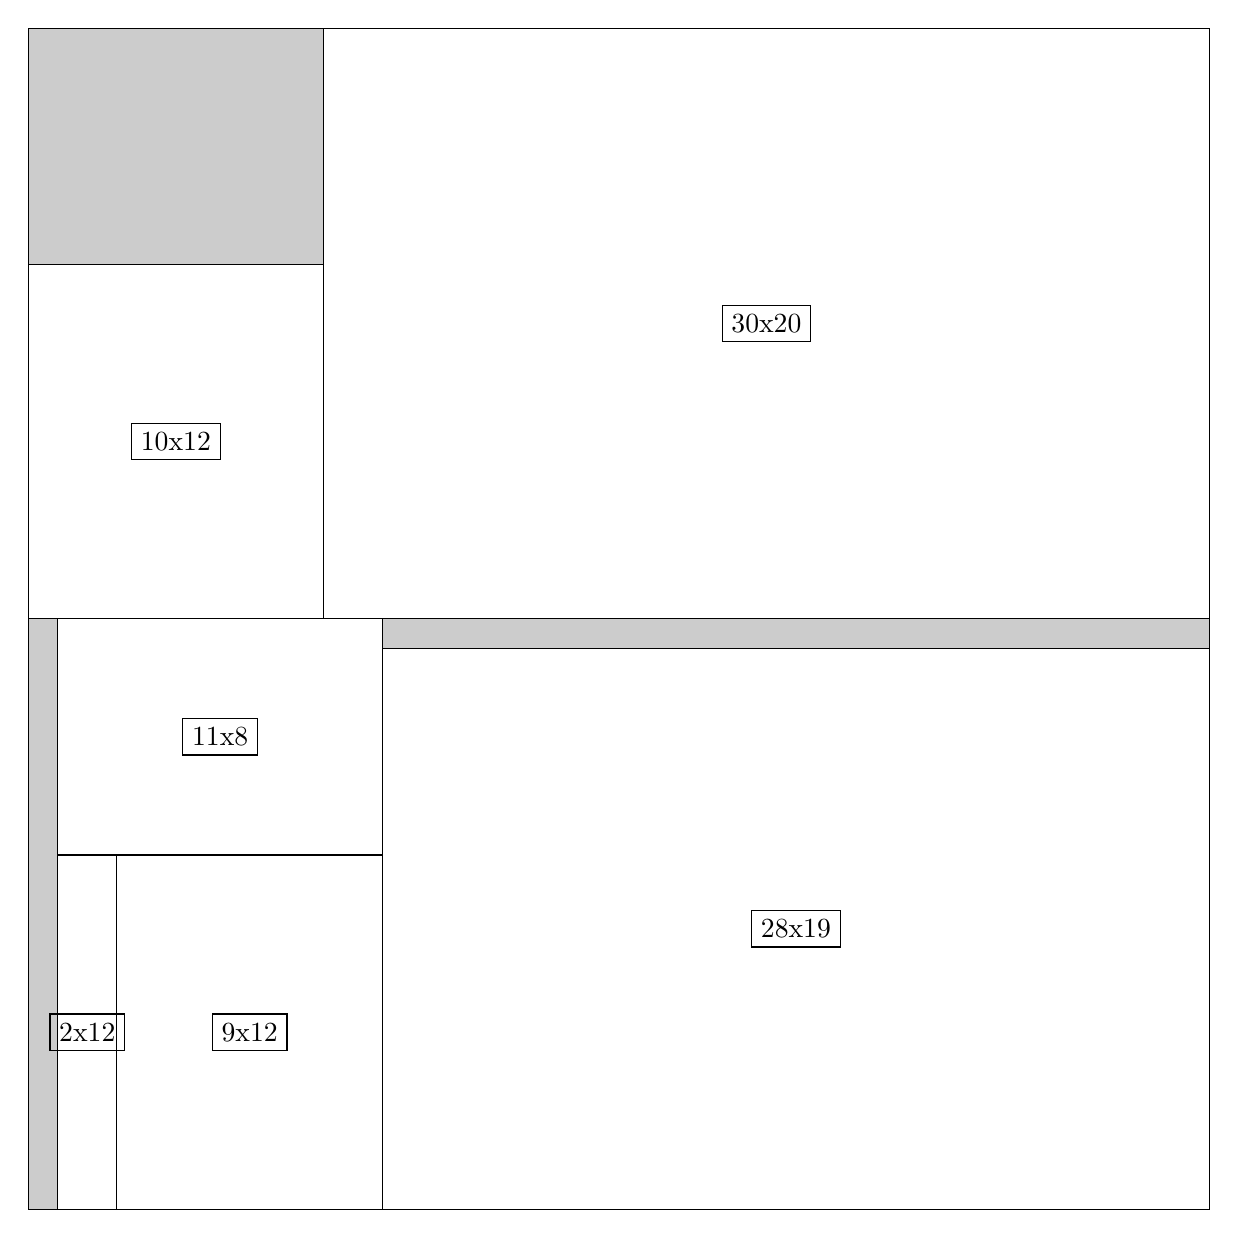
\begin{tikzpicture}[shorten >=1pt,scale=1.0,every node/.style={scale=1.0},->]
\tikzstyle{vertex}=[circle,fill=black!25,minimum size=14pt,inner sep=0pt]
\filldraw[fill=gray!40!white, draw=black] (0,0) rectangle (15.0,15.0);
\foreach \name/\x/\y/\w/\h in {28x19/4.5/0.0/10.5/7.125,9x12/1.125/0.0/3.375/4.5,2x12/0.375/0.0/0.75/4.5,11x8/0.375/4.5/4.125/3.0,30x20/3.75/7.5/11.25/7.5,10x12/0.0/7.5/3.75/4.5}
\filldraw[fill=white!40!white, draw=black] (\x,\y) rectangle node[draw] (\name) {\name} ++(\w,\h);
\end{tikzpicture}


w =28 , h =19 , x =12 , y =0 , v =532
\par
w =9 , h =12 , x =3 , y =0 , v =108
\par
w =2 , h =12 , x =1 , y =0 , v =24
\par
w =11 , h =8 , x =1 , y =12 , v =88
\par
w =30 , h =20 , x =10 , y =20 , v =600
\par
w =10 , h =12 , x =0 , y =20 , v =120
\par
\newpage


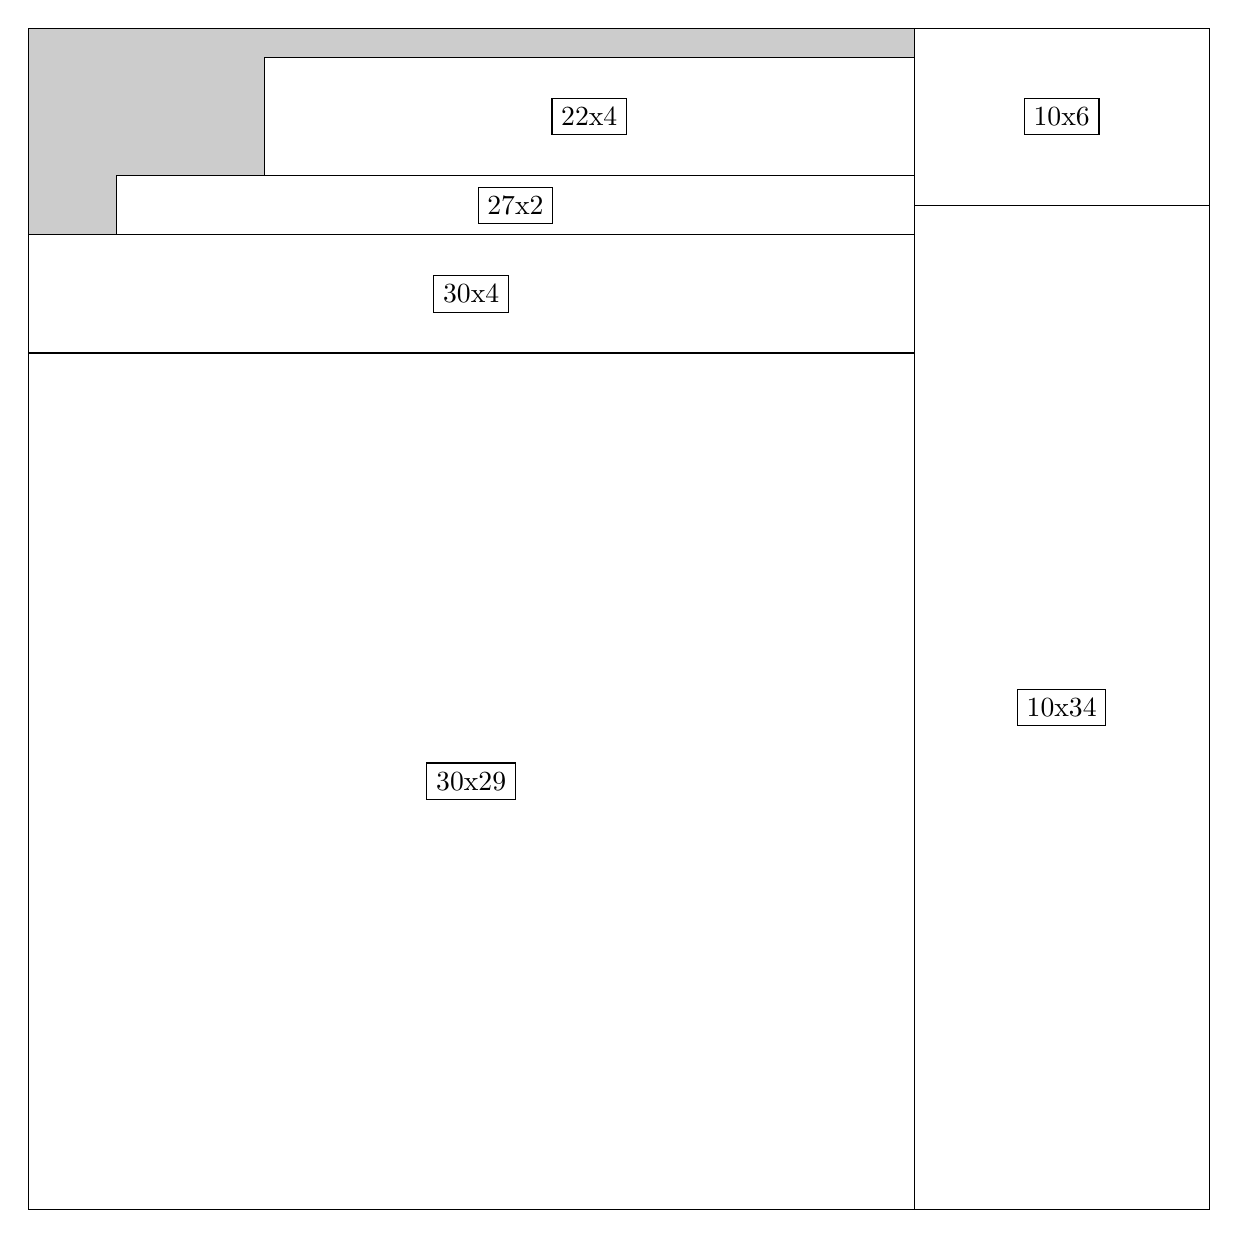
\begin{tikzpicture}[shorten >=1pt,scale=1.0,every node/.style={scale=1.0},->]
\tikzstyle{vertex}=[circle,fill=black!25,minimum size=14pt,inner sep=0pt]
\filldraw[fill=gray!40!white, draw=black] (0,0) rectangle (15.0,15.0);
\foreach \name/\x/\y/\w/\h in {10x34/11.25/0.0/3.75/12.75,10x6/11.25/12.75/3.75/2.25,30x29/0.0/0.0/11.25/10.875,30x4/0.0/10.875/11.25/1.5,27x2/1.125/12.375/10.125/0.75,22x4/3.0/13.125/8.25/1.5}
\filldraw[fill=white!40!white, draw=black] (\x,\y) rectangle node[draw] (\name) {\name} ++(\w,\h);
\end{tikzpicture}


w =10 , h =34 , x =30 , y =0 , v =340
\par
w =10 , h =6 , x =30 , y =34 , v =60
\par
w =30 , h =29 , x =0 , y =0 , v =870
\par
w =30 , h =4 , x =0 , y =29 , v =120
\par
w =27 , h =2 , x =3 , y =33 , v =54
\par
w =22 , h =4 , x =8 , y =35 , v =88
\par
\newpage


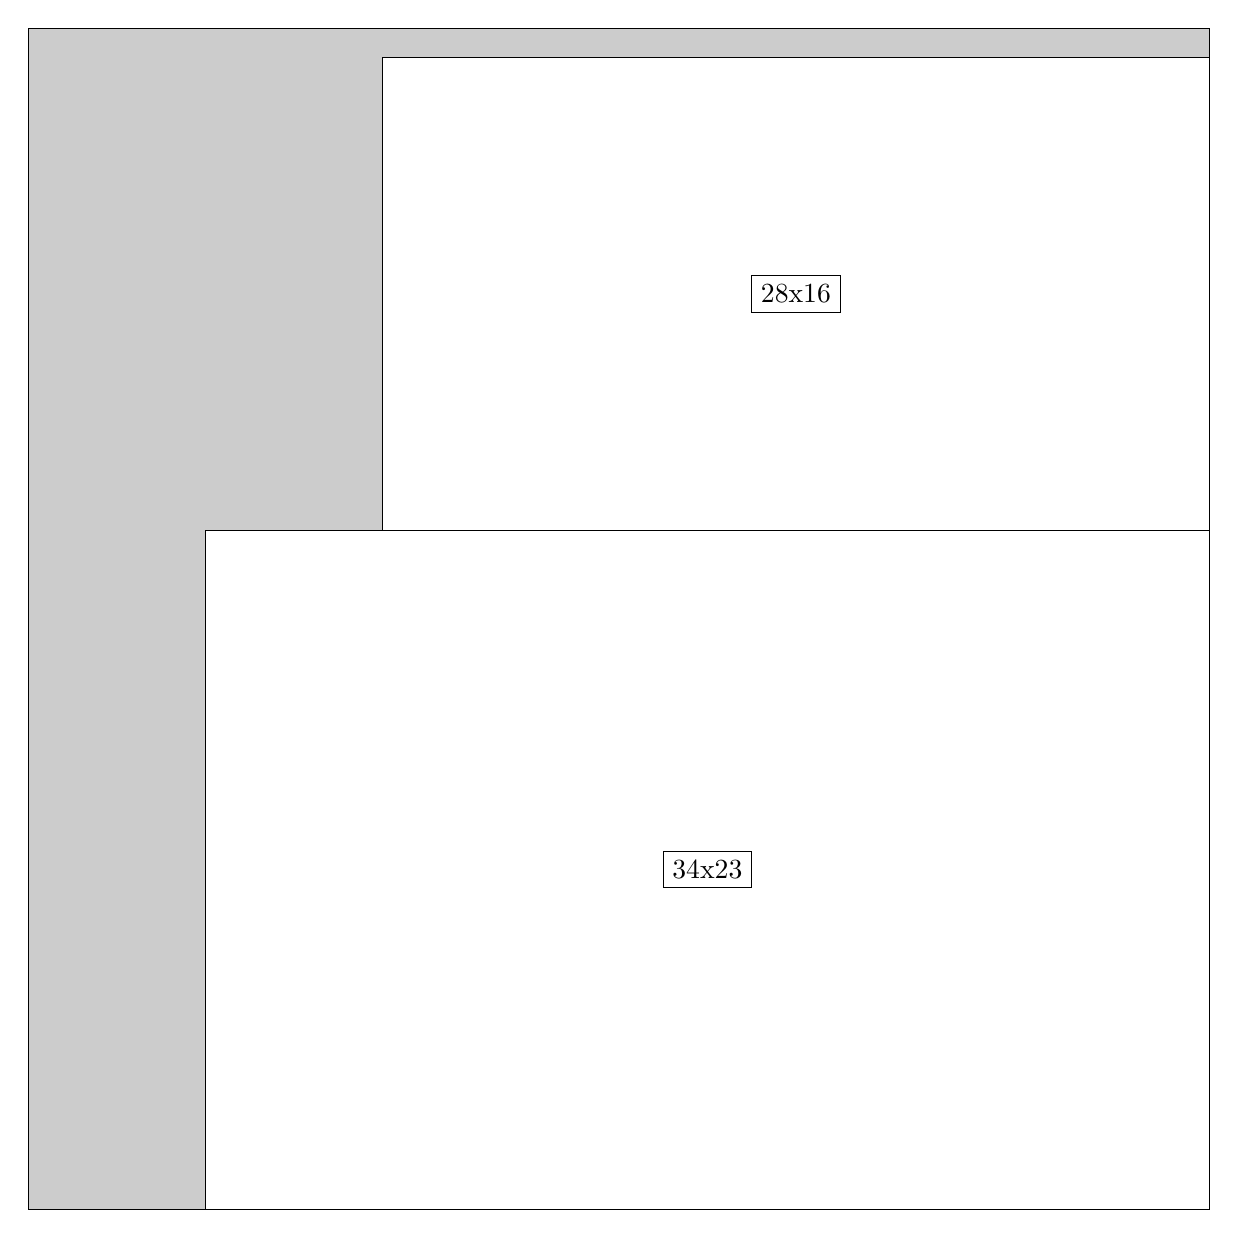
\begin{tikzpicture}[shorten >=1pt,scale=1.0,every node/.style={scale=1.0},->]
\tikzstyle{vertex}=[circle,fill=black!25,minimum size=14pt,inner sep=0pt]
\filldraw[fill=gray!40!white, draw=black] (0,0) rectangle (15.0,15.0);
\foreach \name/\x/\y/\w/\h in {34x23/2.25/0.0/12.75/8.625,28x16/4.5/8.625/10.5/6.0}
\filldraw[fill=white!40!white, draw=black] (\x,\y) rectangle node[draw] (\name) {\name} ++(\w,\h);
\end{tikzpicture}


w =34 , h =23 , x =6 , y =0 , v =782
\par
w =28 , h =16 , x =12 , y =23 , v =448
\par
\newpage


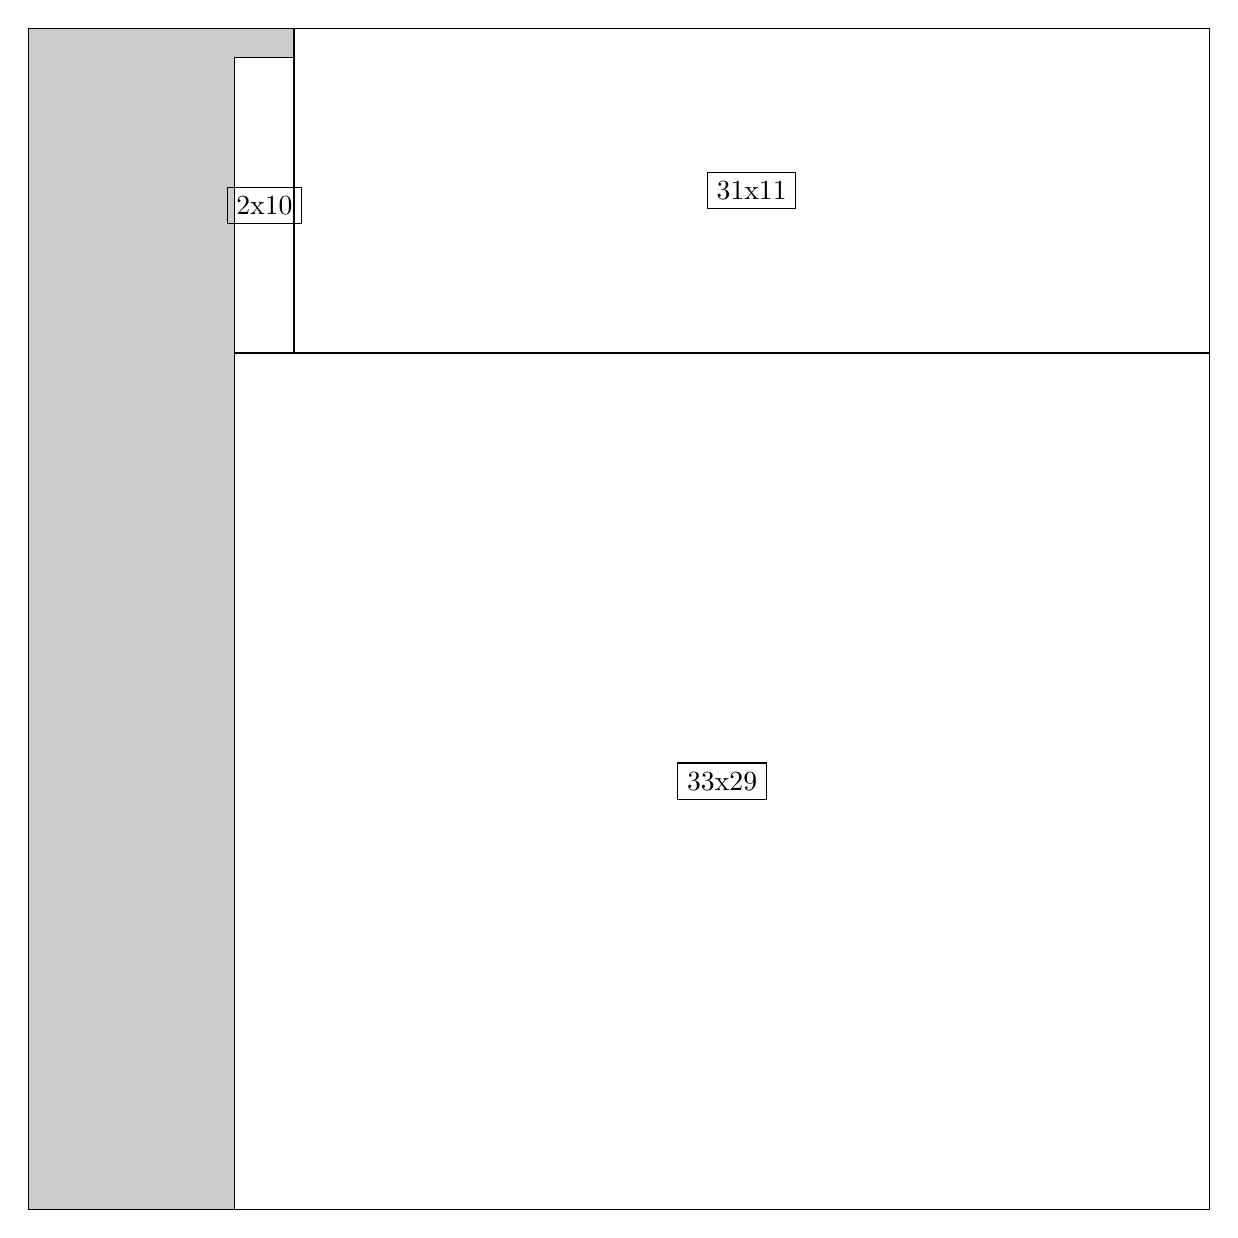
\begin{tikzpicture}[shorten >=1pt,scale=1.0,every node/.style={scale=1.0},->]
\tikzstyle{vertex}=[circle,fill=black!25,minimum size=14pt,inner sep=0pt]
\filldraw[fill=gray!40!white, draw=black] (0,0) rectangle (15.0,15.0);
\foreach \name/\x/\y/\w/\h in {33x29/2.625/0.0/12.375/10.875,31x11/3.375/10.875/11.625/4.125,2x10/2.625/10.875/0.75/3.75}
\filldraw[fill=white!40!white, draw=black] (\x,\y) rectangle node[draw] (\name) {\name} ++(\w,\h);
\end{tikzpicture}


w =33 , h =29 , x =7 , y =0 , v =957
\par
w =31 , h =11 , x =9 , y =29 , v =341
\par
w =2 , h =10 , x =7 , y =29 , v =20
\par
\newpage


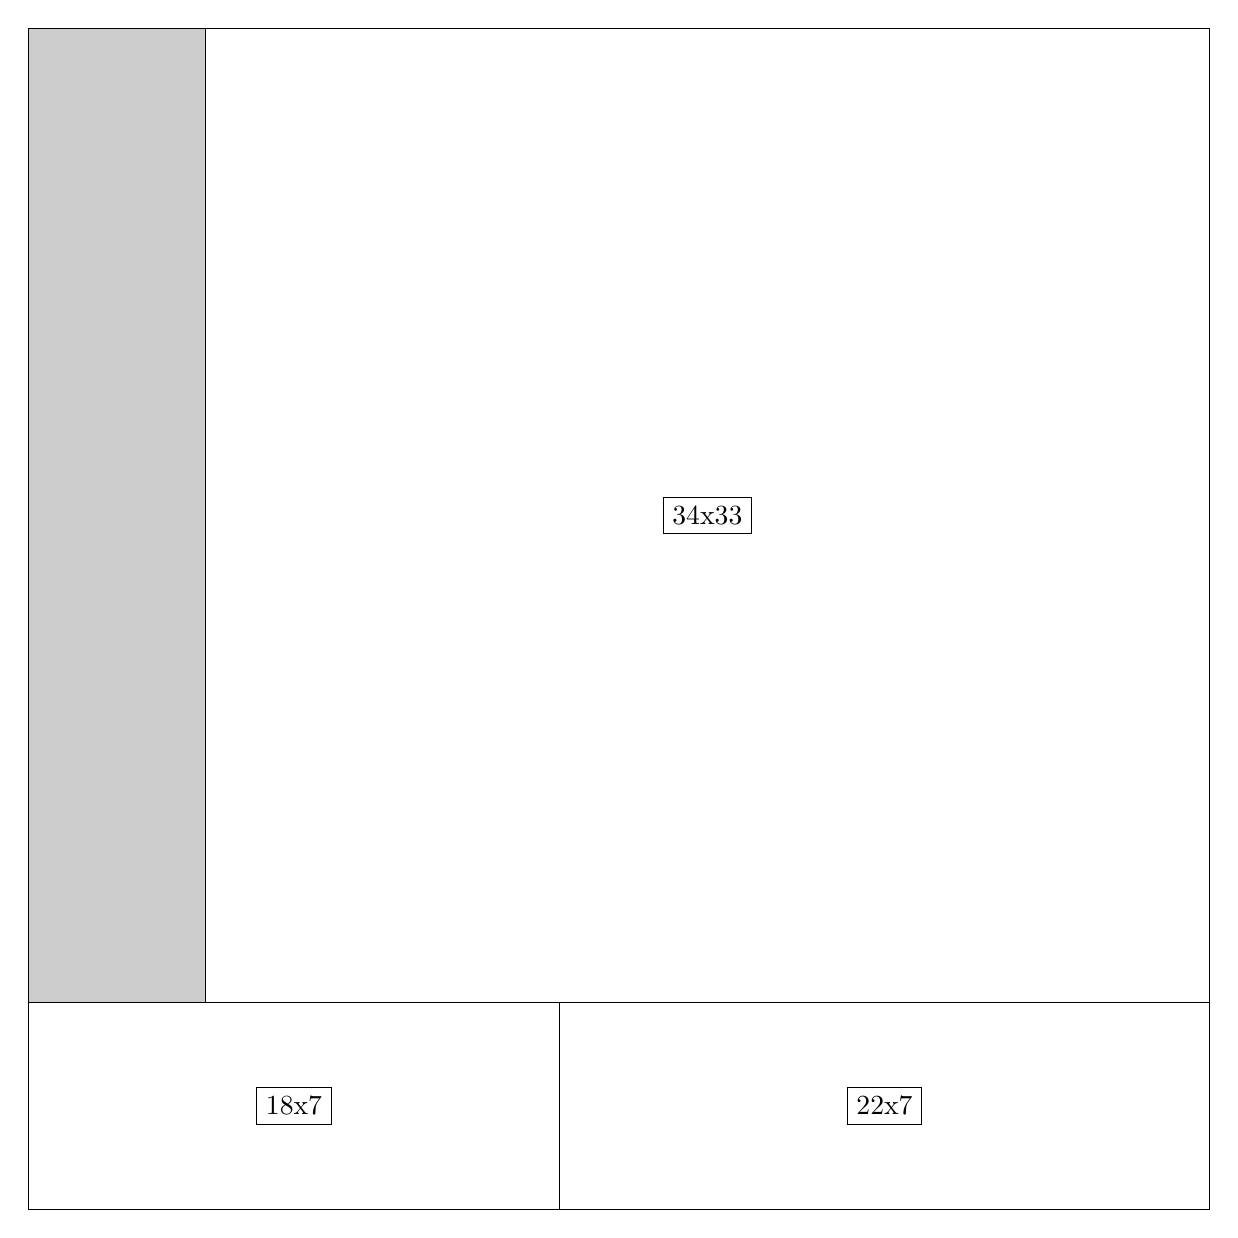
\begin{tikzpicture}[shorten >=1pt,scale=1.0,every node/.style={scale=1.0},->]
\tikzstyle{vertex}=[circle,fill=black!25,minimum size=14pt,inner sep=0pt]
\filldraw[fill=gray!40!white, draw=black] (0,0) rectangle (15.0,15.0);
\foreach \name/\x/\y/\w/\h in {22x7/6.75/0.0/8.25/2.625,18x7/0.0/0.0/6.75/2.625,34x33/2.25/2.625/12.75/12.375}
\filldraw[fill=white!40!white, draw=black] (\x,\y) rectangle node[draw] (\name) {\name} ++(\w,\h);
\end{tikzpicture}


w =22 , h =7 , x =18 , y =0 , v =154
\par
w =18 , h =7 , x =0 , y =0 , v =126
\par
w =34 , h =33 , x =6 , y =7 , v =1122
\par
\newpage


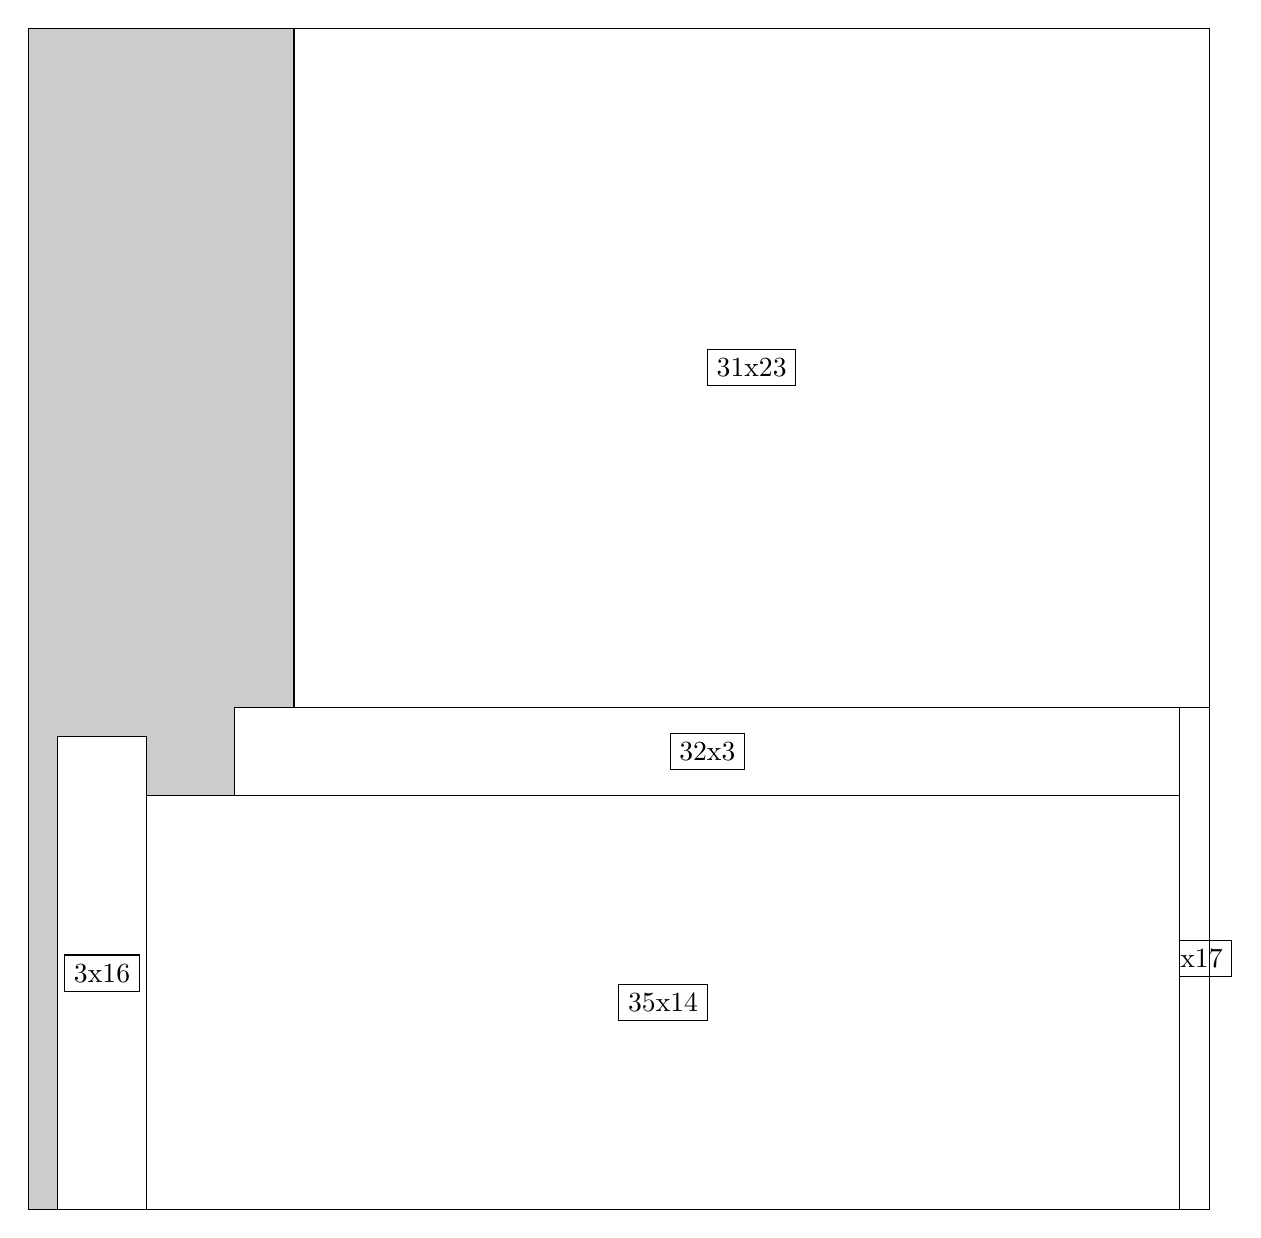
\begin{tikzpicture}[shorten >=1pt,scale=1.0,every node/.style={scale=1.0},->]
\tikzstyle{vertex}=[circle,fill=black!25,minimum size=14pt,inner sep=0pt]
\filldraw[fill=gray!40!white, draw=black] (0,0) rectangle (15.0,15.0);
\foreach \name/\x/\y/\w/\h in {1x17/14.625/0.0/0.375/6.375,35x14/1.5/0.0/13.125/5.25,32x3/2.625/5.25/12.0/1.125,3x16/0.375/0.0/1.125/6.0,31x23/3.375/6.375/11.625/8.625}
\filldraw[fill=white!40!white, draw=black] (\x,\y) rectangle node[draw] (\name) {\name} ++(\w,\h);
\end{tikzpicture}


w =1 , h =17 , x =39 , y =0 , v =17
\par
w =35 , h =14 , x =4 , y =0 , v =490
\par
w =32 , h =3 , x =7 , y =14 , v =96
\par
w =3 , h =16 , x =1 , y =0 , v =48
\par
w =31 , h =23 , x =9 , y =17 , v =713
\par
\newpage


\begin{tikzpicture}[shorten >=1pt,scale=1.0,every node/.style={scale=1.0},->]
\tikzstyle{vertex}=[circle,fill=black!25,minimum size=14pt,inner sep=0pt]
\filldraw[fill=gray!40!white, draw=black] (0,0) rectangle (15.0,15.0);
\foreach \name/\x/\y/\w/\h in {28x30/4.5/0.0/10.5/11.25,9x30/1.125/0.0/3.375/11.25,3x30/0.0/0.0/1.125/11.25,17x10/8.625/11.25/6.375/3.75,23x5/0.0/11.25/8.625/1.875,21x5/0.75/13.125/7.875/1.875}
\filldraw[fill=white!40!white, draw=black] (\x,\y) rectangle node[draw] (\name) {\name} ++(\w,\h);
\end{tikzpicture}


w =28 , h =30 , x =12 , y =0 , v =840
\par
w =9 , h =30 , x =3 , y =0 , v =270
\par
w =3 , h =30 , x =0 , y =0 , v =90
\par
w =17 , h =10 , x =23 , y =30 , v =170
\par
w =23 , h =5 , x =0 , y =30 , v =115
\par
w =21 , h =5 , x =2 , y =35 , v =105
\par
\newpage


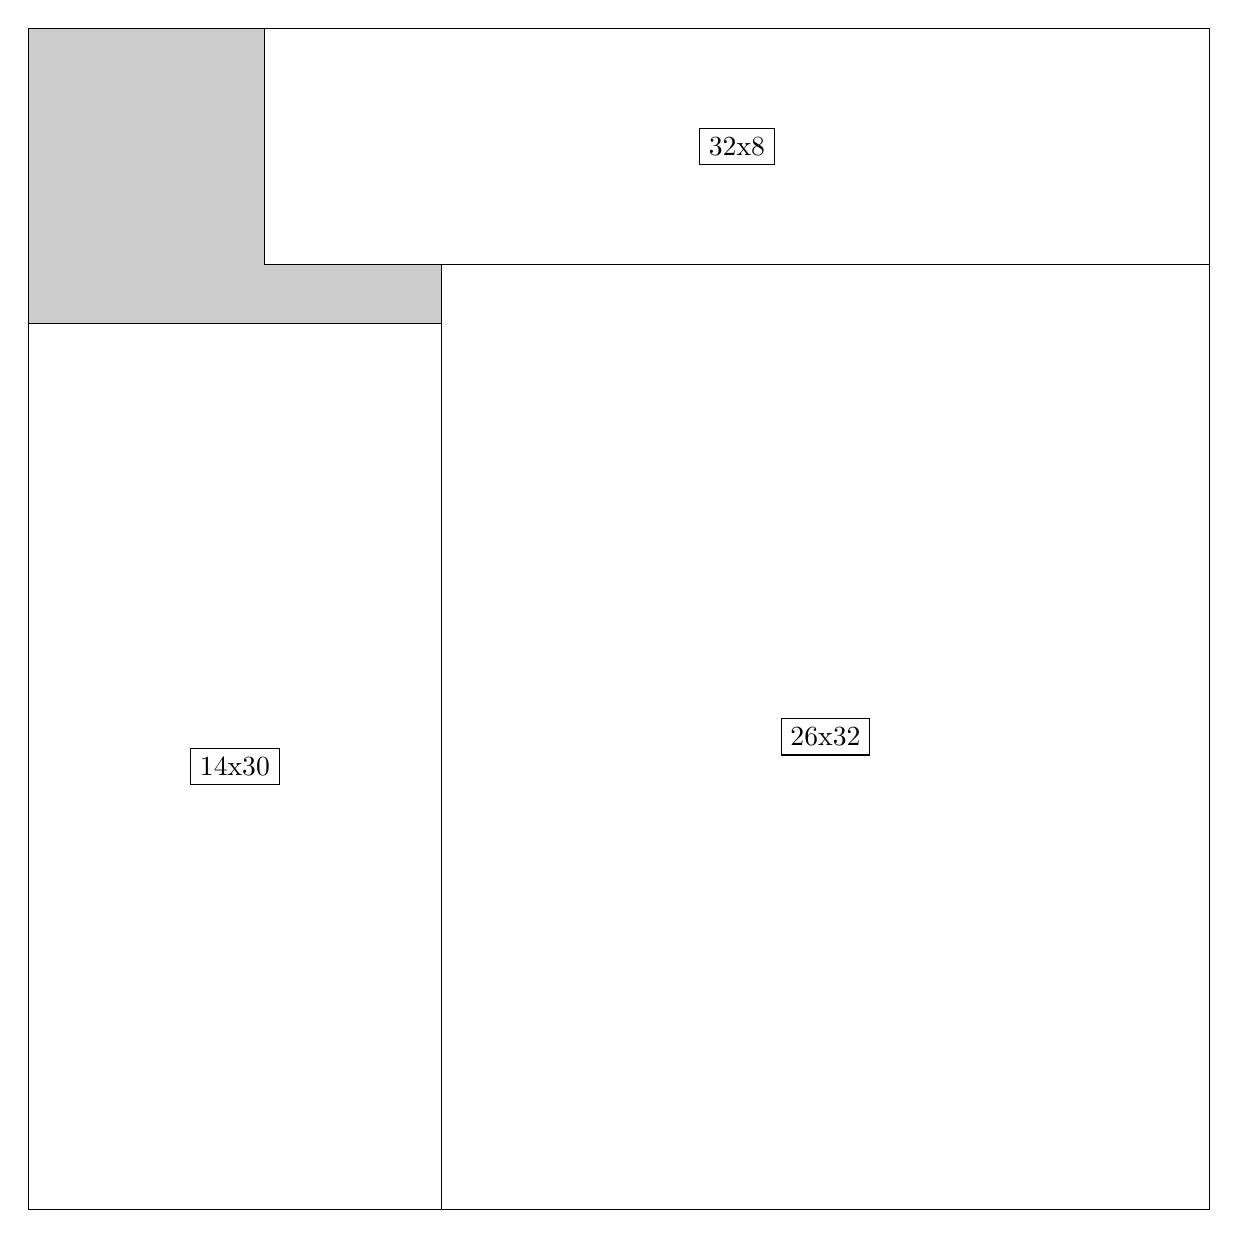
\begin{tikzpicture}[shorten >=1pt,scale=1.0,every node/.style={scale=1.0},->]
\tikzstyle{vertex}=[circle,fill=black!25,minimum size=14pt,inner sep=0pt]
\filldraw[fill=gray!40!white, draw=black] (0,0) rectangle (15.0,15.0);
\foreach \name/\x/\y/\w/\h in {26x32/5.25/0.0/9.75/12.0,14x30/0.0/0.0/5.25/11.25,32x8/3.0/12.0/12.0/3.0}
\filldraw[fill=white!40!white, draw=black] (\x,\y) rectangle node[draw] (\name) {\name} ++(\w,\h);
\end{tikzpicture}


w =26 , h =32 , x =14 , y =0 , v =832
\par
w =14 , h =30 , x =0 , y =0 , v =420
\par
w =32 , h =8 , x =8 , y =32 , v =256
\par
\newpage


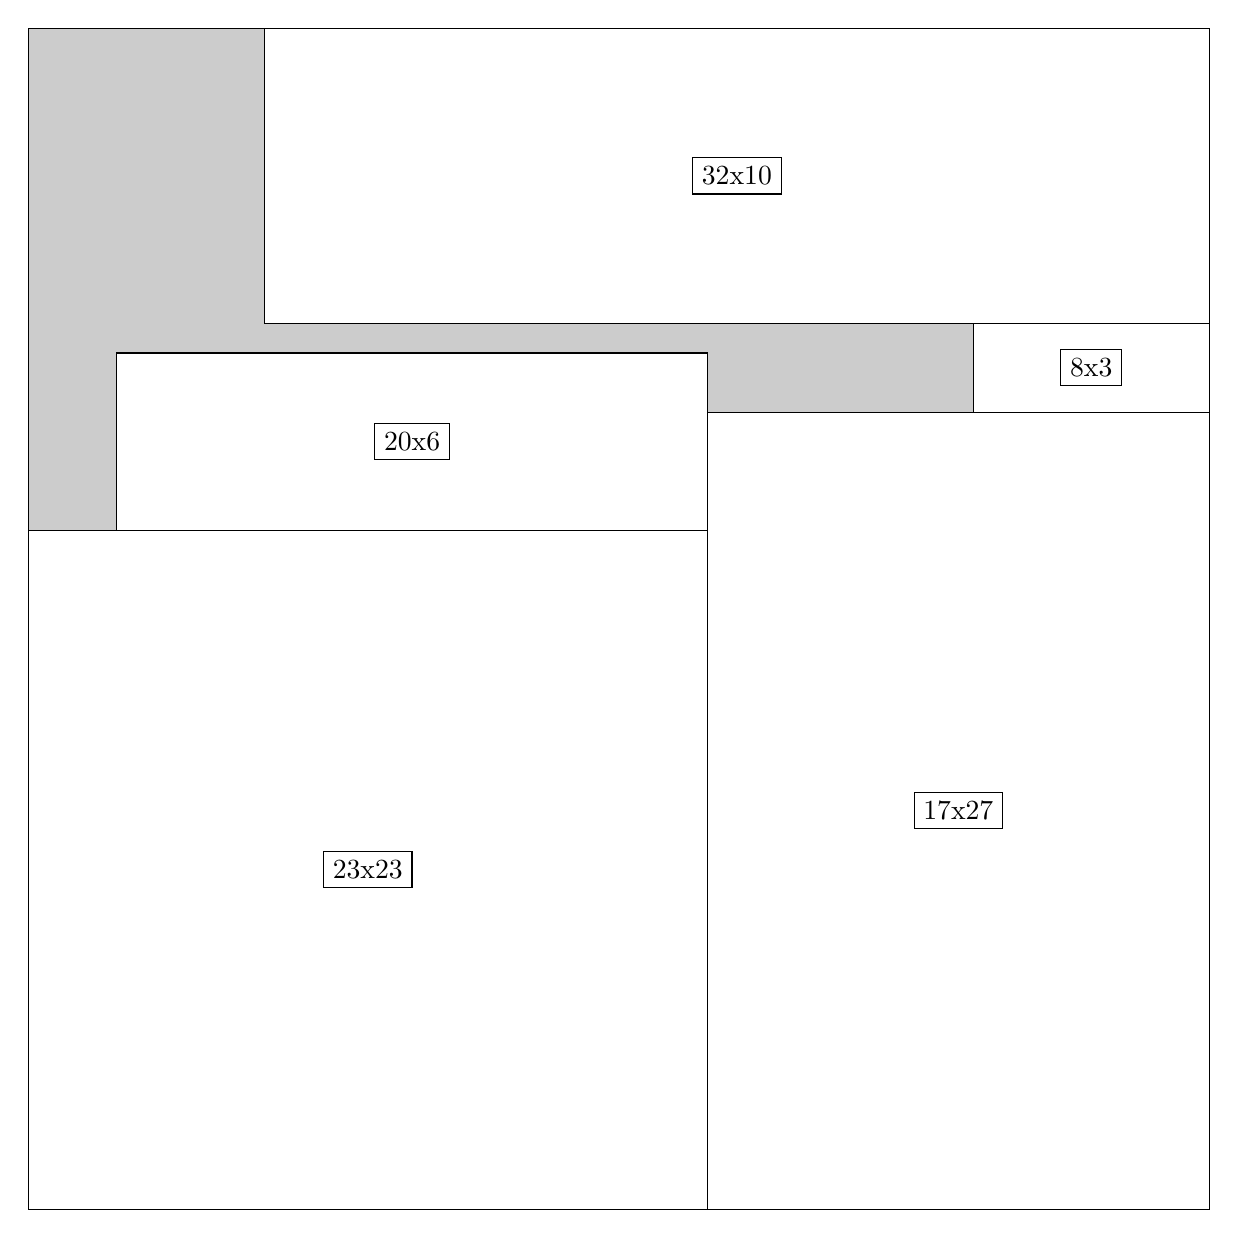
\begin{tikzpicture}[shorten >=1pt,scale=1.0,every node/.style={scale=1.0},->]
\tikzstyle{vertex}=[circle,fill=black!25,minimum size=14pt,inner sep=0pt]
\filldraw[fill=gray!40!white, draw=black] (0,0) rectangle (15.0,15.0);
\foreach \name/\x/\y/\w/\h in {17x27/8.625/0.0/6.375/10.125,8x3/12.0/10.125/3.0/1.125,23x23/0.0/0.0/8.625/8.625,20x6/1.125/8.625/7.5/2.25,32x10/3.0/11.25/12.0/3.75}
\filldraw[fill=white!40!white, draw=black] (\x,\y) rectangle node[draw] (\name) {\name} ++(\w,\h);
\end{tikzpicture}


w =17 , h =27 , x =23 , y =0 , v =459
\par
w =8 , h =3 , x =32 , y =27 , v =24
\par
w =23 , h =23 , x =0 , y =0 , v =529
\par
w =20 , h =6 , x =3 , y =23 , v =120
\par
w =32 , h =10 , x =8 , y =30 , v =320
\par
\newpage


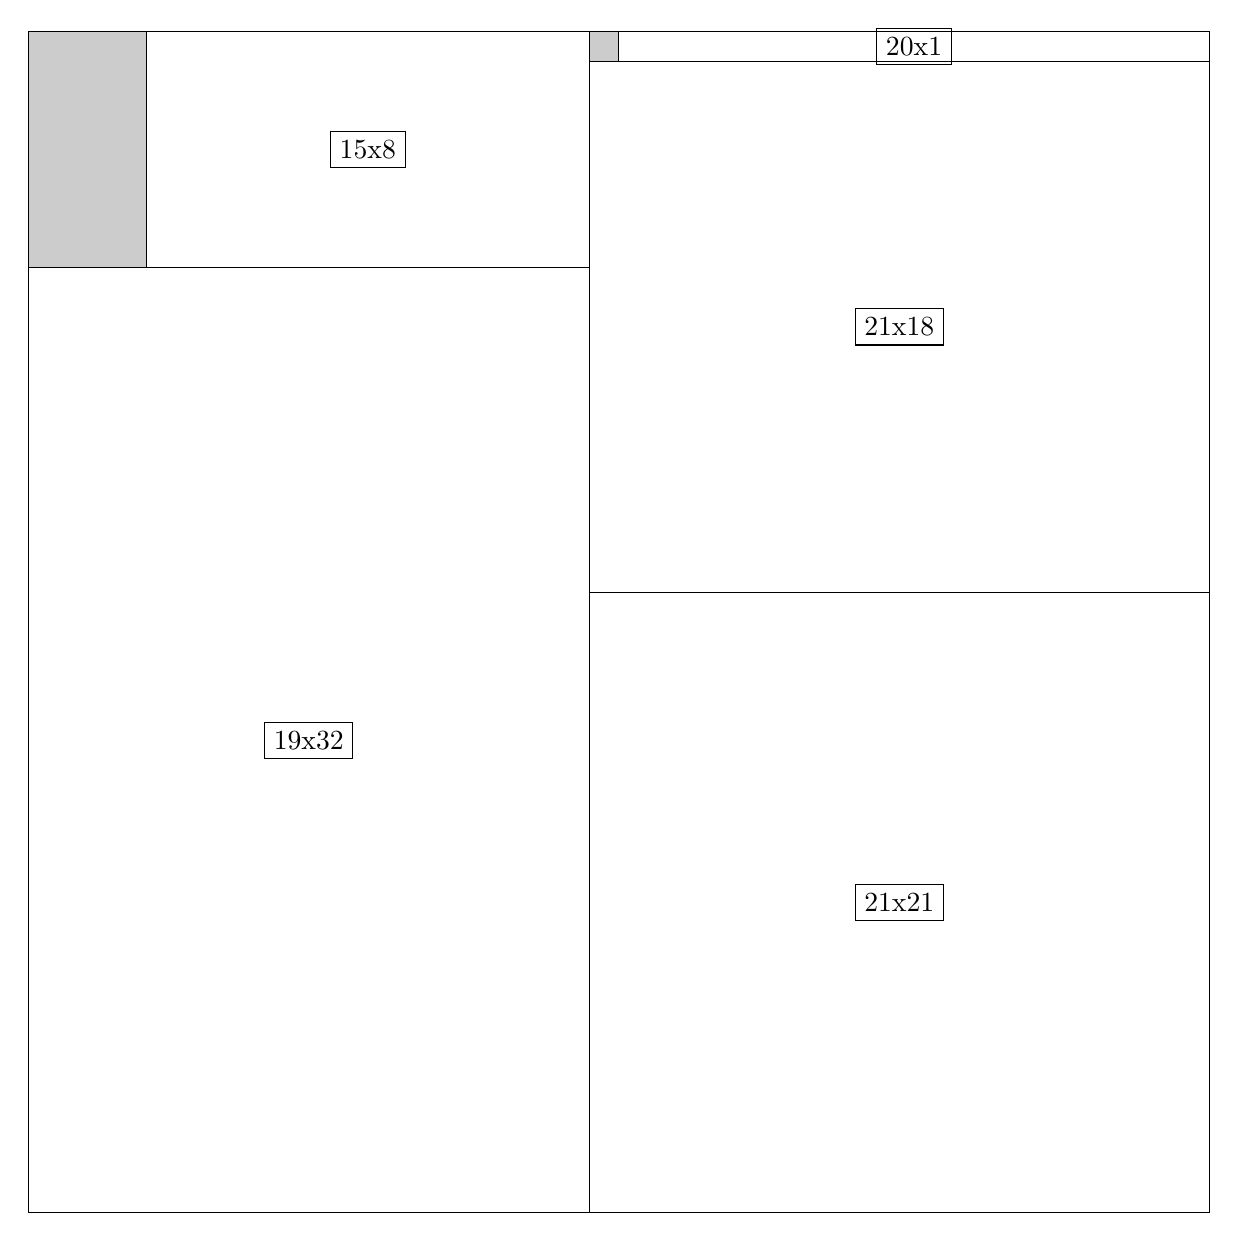
\begin{tikzpicture}[shorten >=1pt,scale=1.0,every node/.style={scale=1.0},->]
\tikzstyle{vertex}=[circle,fill=black!25,minimum size=14pt,inner sep=0pt]
\filldraw[fill=gray!40!white, draw=black] (0,0) rectangle (15.0,15.0);
\foreach \name/\x/\y/\w/\h in {21x21/7.125/0.0/7.875/7.875,21x18/7.125/7.875/7.875/6.75,20x1/7.5/14.625/7.5/0.375,19x32/0.0/0.0/7.125/12.0,15x8/1.5/12.0/5.625/3.0}
\filldraw[fill=white!40!white, draw=black] (\x,\y) rectangle node[draw] (\name) {\name} ++(\w,\h);
\end{tikzpicture}


w =21 , h =21 , x =19 , y =0 , v =441
\par
w =21 , h =18 , x =19 , y =21 , v =378
\par
w =20 , h =1 , x =20 , y =39 , v =20
\par
w =19 , h =32 , x =0 , y =0 , v =608
\par
w =15 , h =8 , x =4 , y =32 , v =120
\par
\newpage


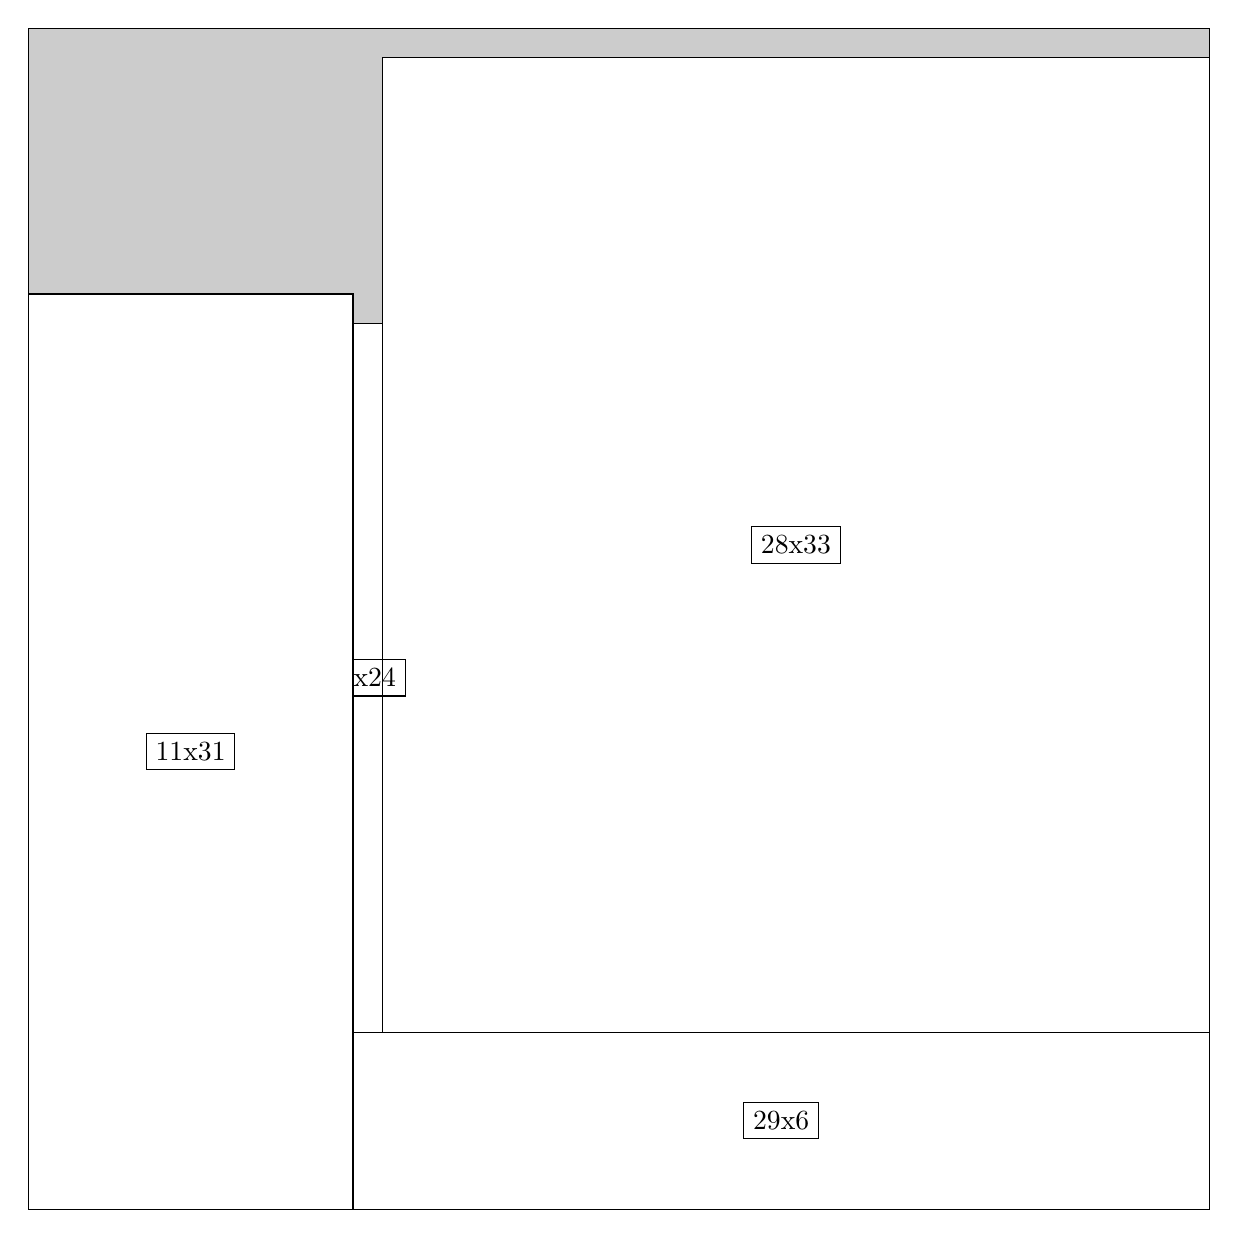
\begin{tikzpicture}[shorten >=1pt,scale=1.0,every node/.style={scale=1.0},->]
\tikzstyle{vertex}=[circle,fill=black!25,minimum size=14pt,inner sep=0pt]
\filldraw[fill=gray!40!white, draw=black] (0,0) rectangle (15.0,15.0);
\foreach \name/\x/\y/\w/\h in {29x6/4.125/0.0/10.875/2.25,28x33/4.5/2.25/10.5/12.375,1x24/4.125/2.25/0.375/9.0,11x31/0.0/0.0/4.125/11.625}
\filldraw[fill=white!40!white, draw=black] (\x,\y) rectangle node[draw] (\name) {\name} ++(\w,\h);
\end{tikzpicture}


w =29 , h =6 , x =11 , y =0 , v =174
\par
w =28 , h =33 , x =12 , y =6 , v =924
\par
w =1 , h =24 , x =11 , y =6 , v =24
\par
w =11 , h =31 , x =0 , y =0 , v =341
\par
\newpage


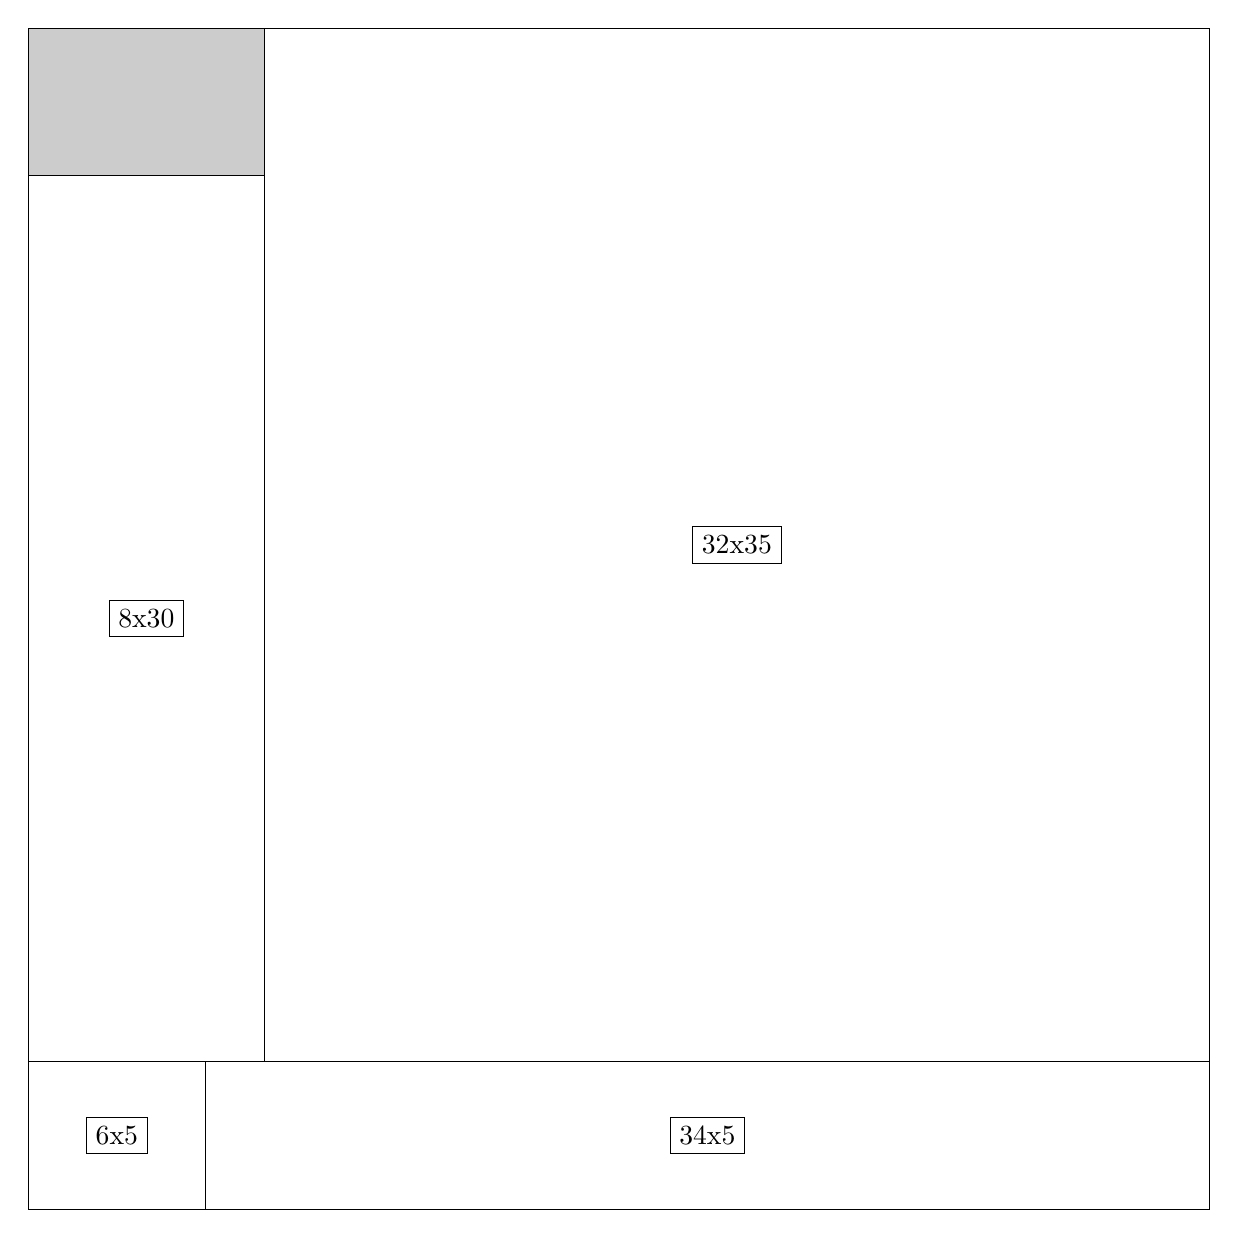
\begin{tikzpicture}[shorten >=1pt,scale=1.0,every node/.style={scale=1.0},->]
\tikzstyle{vertex}=[circle,fill=black!25,minimum size=14pt,inner sep=0pt]
\filldraw[fill=gray!40!white, draw=black] (0,0) rectangle (15.0,15.0);
\foreach \name/\x/\y/\w/\h in {34x5/2.25/0.0/12.75/1.875,6x5/0.0/0.0/2.25/1.875,32x35/3.0/1.875/12.0/13.125,8x30/0.0/1.875/3.0/11.25}
\filldraw[fill=white!40!white, draw=black] (\x,\y) rectangle node[draw] (\name) {\name} ++(\w,\h);
\end{tikzpicture}


w =34 , h =5 , x =6 , y =0 , v =170
\par
w =6 , h =5 , x =0 , y =0 , v =30
\par
w =32 , h =35 , x =8 , y =5 , v =1120
\par
w =8 , h =30 , x =0 , y =5 , v =240
\par
\newpage


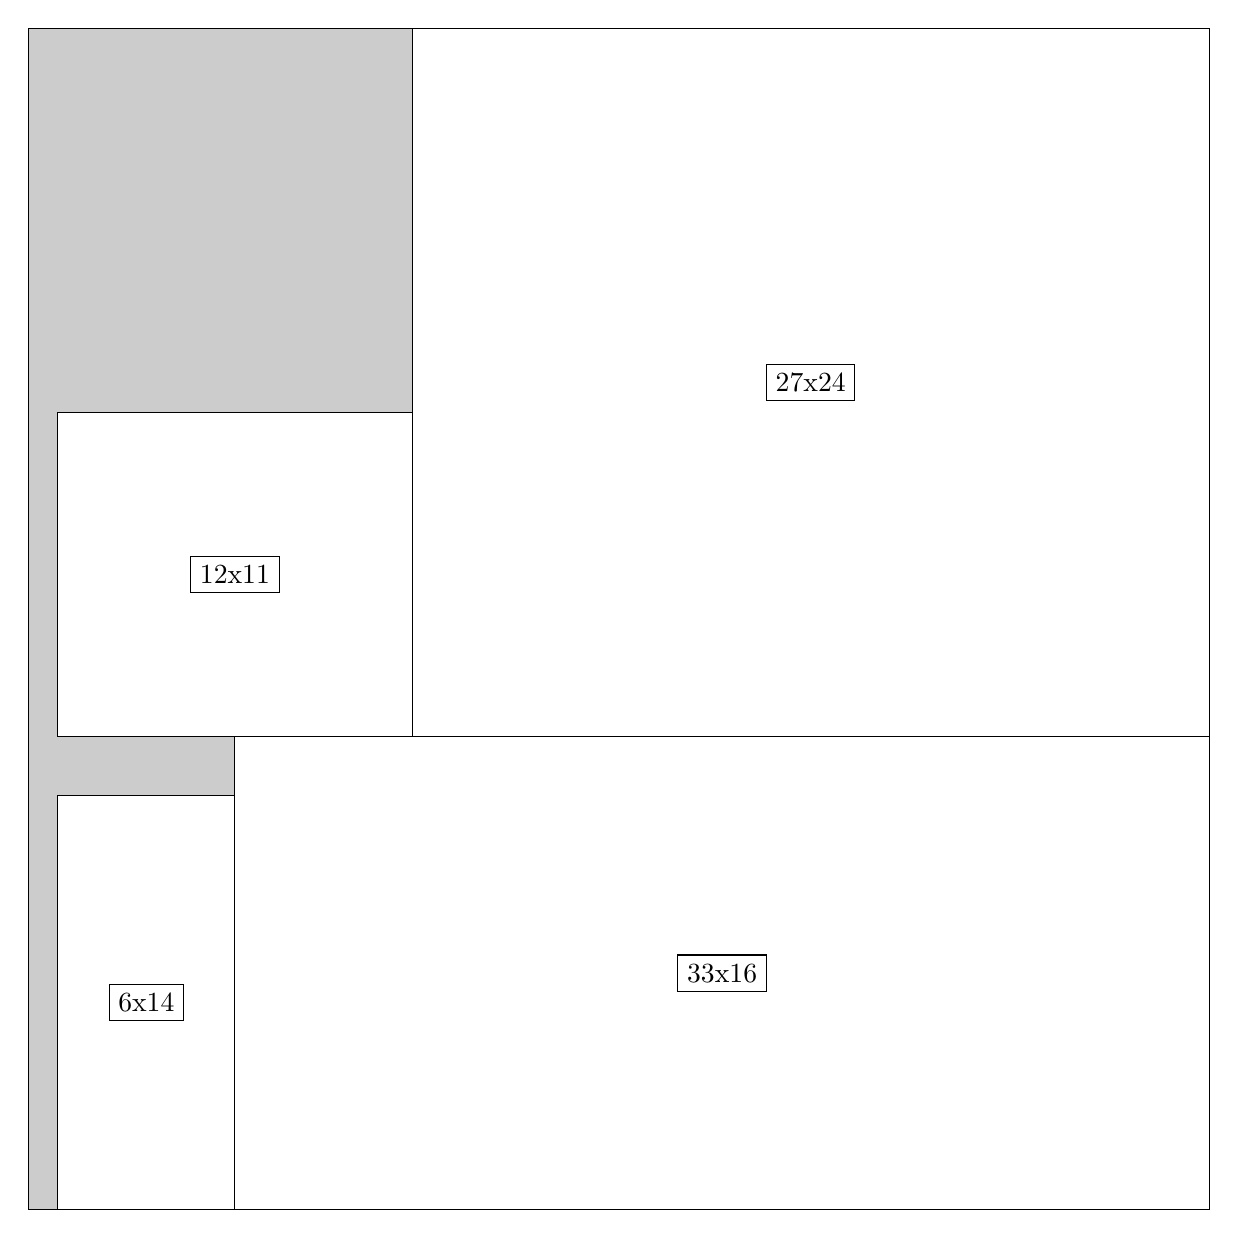
\begin{tikzpicture}[shorten >=1pt,scale=1.0,every node/.style={scale=1.0},->]
\tikzstyle{vertex}=[circle,fill=black!25,minimum size=14pt,inner sep=0pt]
\filldraw[fill=gray!40!white, draw=black] (0,0) rectangle (15.0,15.0);
\foreach \name/\x/\y/\w/\h in {33x16/2.625/0.0/12.375/6.0,6x14/0.375/0.0/2.25/5.25,27x24/4.875/6.0/10.125/9.0,12x11/0.375/6.0/4.5/4.125}
\filldraw[fill=white!40!white, draw=black] (\x,\y) rectangle node[draw] (\name) {\name} ++(\w,\h);
\end{tikzpicture}


w =33 , h =16 , x =7 , y =0 , v =528
\par
w =6 , h =14 , x =1 , y =0 , v =84
\par
w =27 , h =24 , x =13 , y =16 , v =648
\par
w =12 , h =11 , x =1 , y =16 , v =132
\par
\newpage


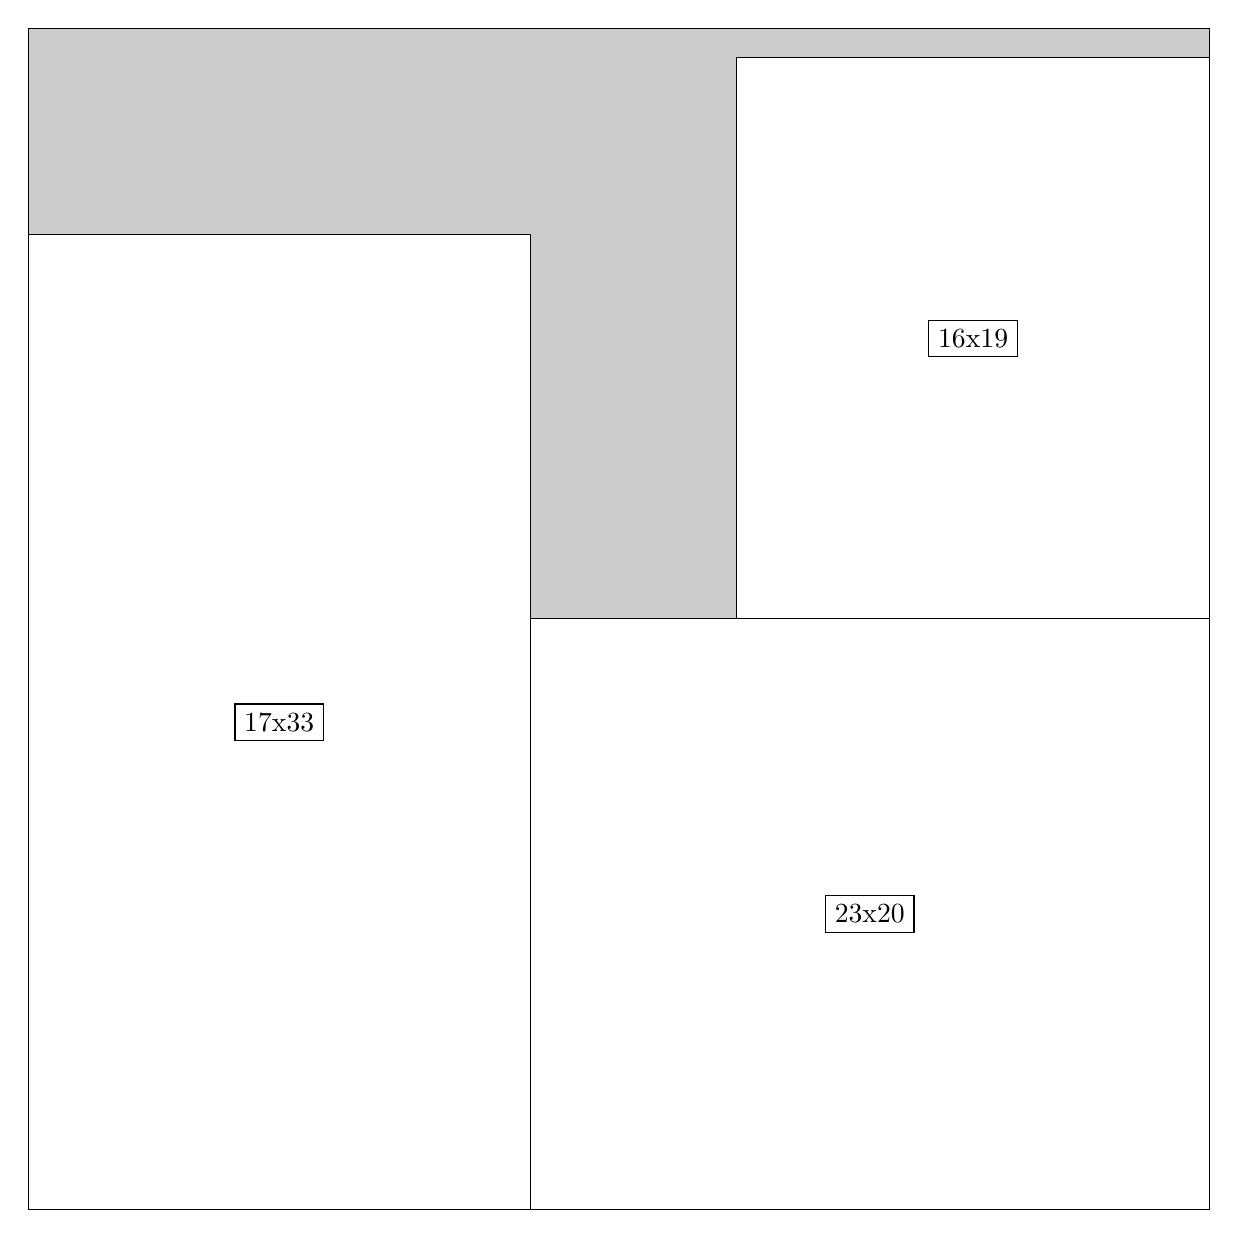
\begin{tikzpicture}[shorten >=1pt,scale=1.0,every node/.style={scale=1.0},->]
\tikzstyle{vertex}=[circle,fill=black!25,minimum size=14pt,inner sep=0pt]
\filldraw[fill=gray!40!white, draw=black] (0,0) rectangle (15.0,15.0);
\foreach \name/\x/\y/\w/\h in {23x20/6.375/0.0/8.625/7.5,16x19/9.0/7.5/6.0/7.125,17x33/0.0/0.0/6.375/12.375}
\filldraw[fill=white!40!white, draw=black] (\x,\y) rectangle node[draw] (\name) {\name} ++(\w,\h);
\end{tikzpicture}


w =23 , h =20 , x =17 , y =0 , v =460
\par
w =16 , h =19 , x =24 , y =20 , v =304
\par
w =17 , h =33 , x =0 , y =0 , v =561
\par
\newpage


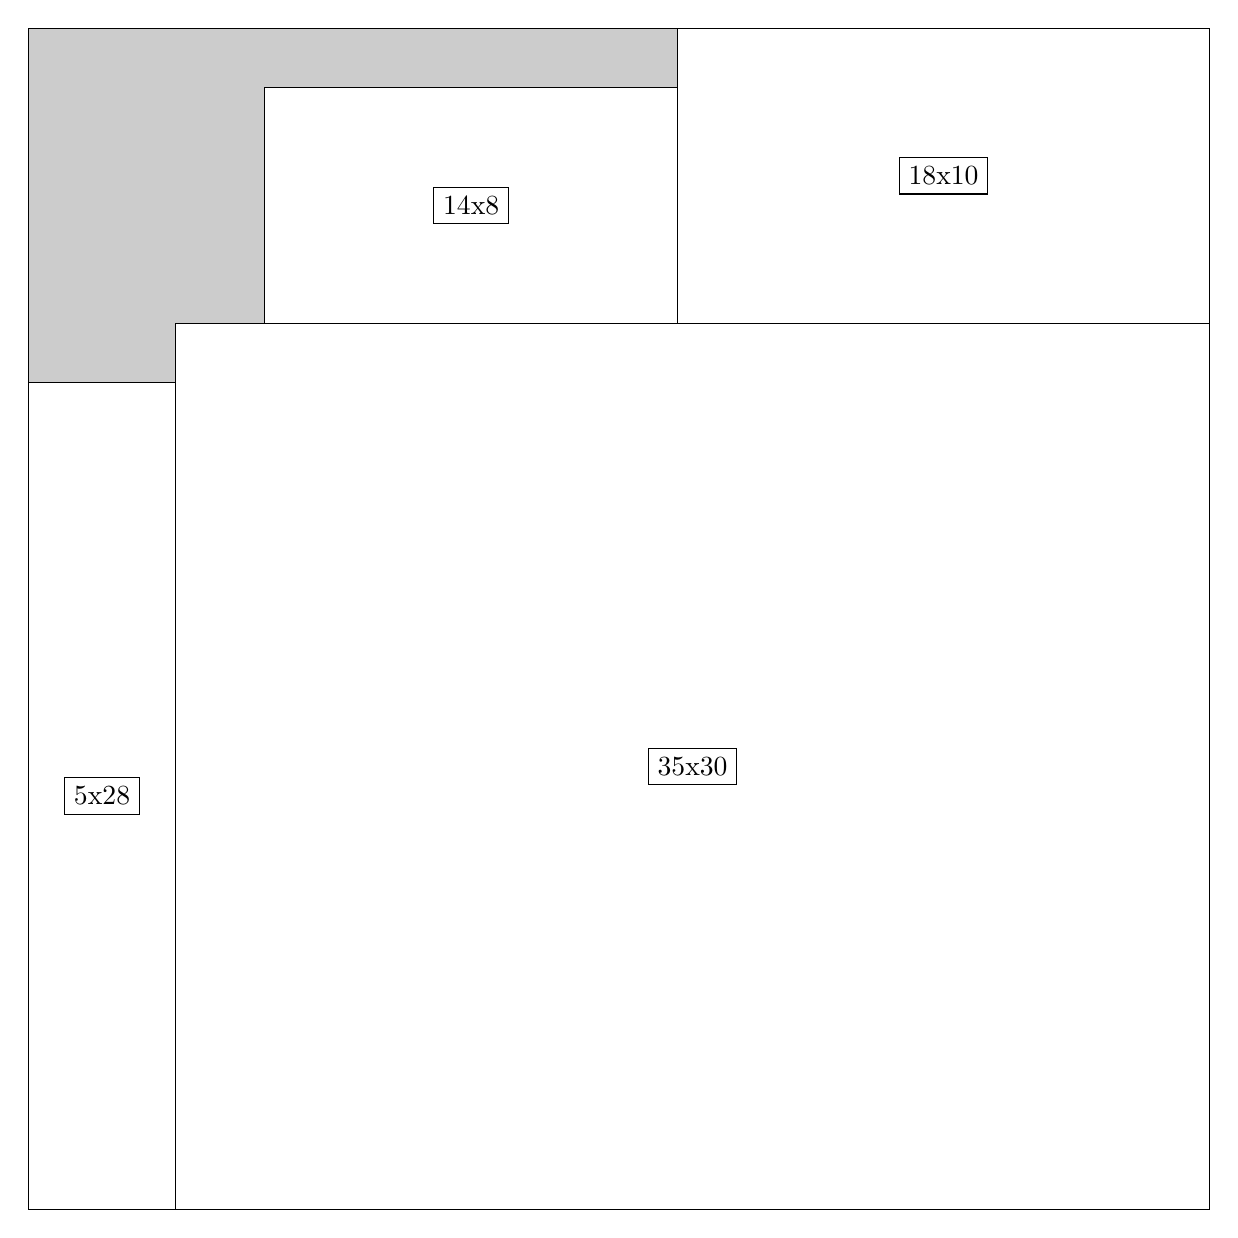
\begin{tikzpicture}[shorten >=1pt,scale=1.0,every node/.style={scale=1.0},->]
\tikzstyle{vertex}=[circle,fill=black!25,minimum size=14pt,inner sep=0pt]
\filldraw[fill=gray!40!white, draw=black] (0,0) rectangle (15.0,15.0);
\foreach \name/\x/\y/\w/\h in {35x30/1.875/0.0/13.125/11.25,5x28/0.0/0.0/1.875/10.5,18x10/8.25/11.25/6.75/3.75,14x8/3.0/11.25/5.25/3.0}
\filldraw[fill=white!40!white, draw=black] (\x,\y) rectangle node[draw] (\name) {\name} ++(\w,\h);
\end{tikzpicture}


w =35 , h =30 , x =5 , y =0 , v =1050
\par
w =5 , h =28 , x =0 , y =0 , v =140
\par
w =18 , h =10 , x =22 , y =30 , v =180
\par
w =14 , h =8 , x =8 , y =30 , v =112
\par
\newpage


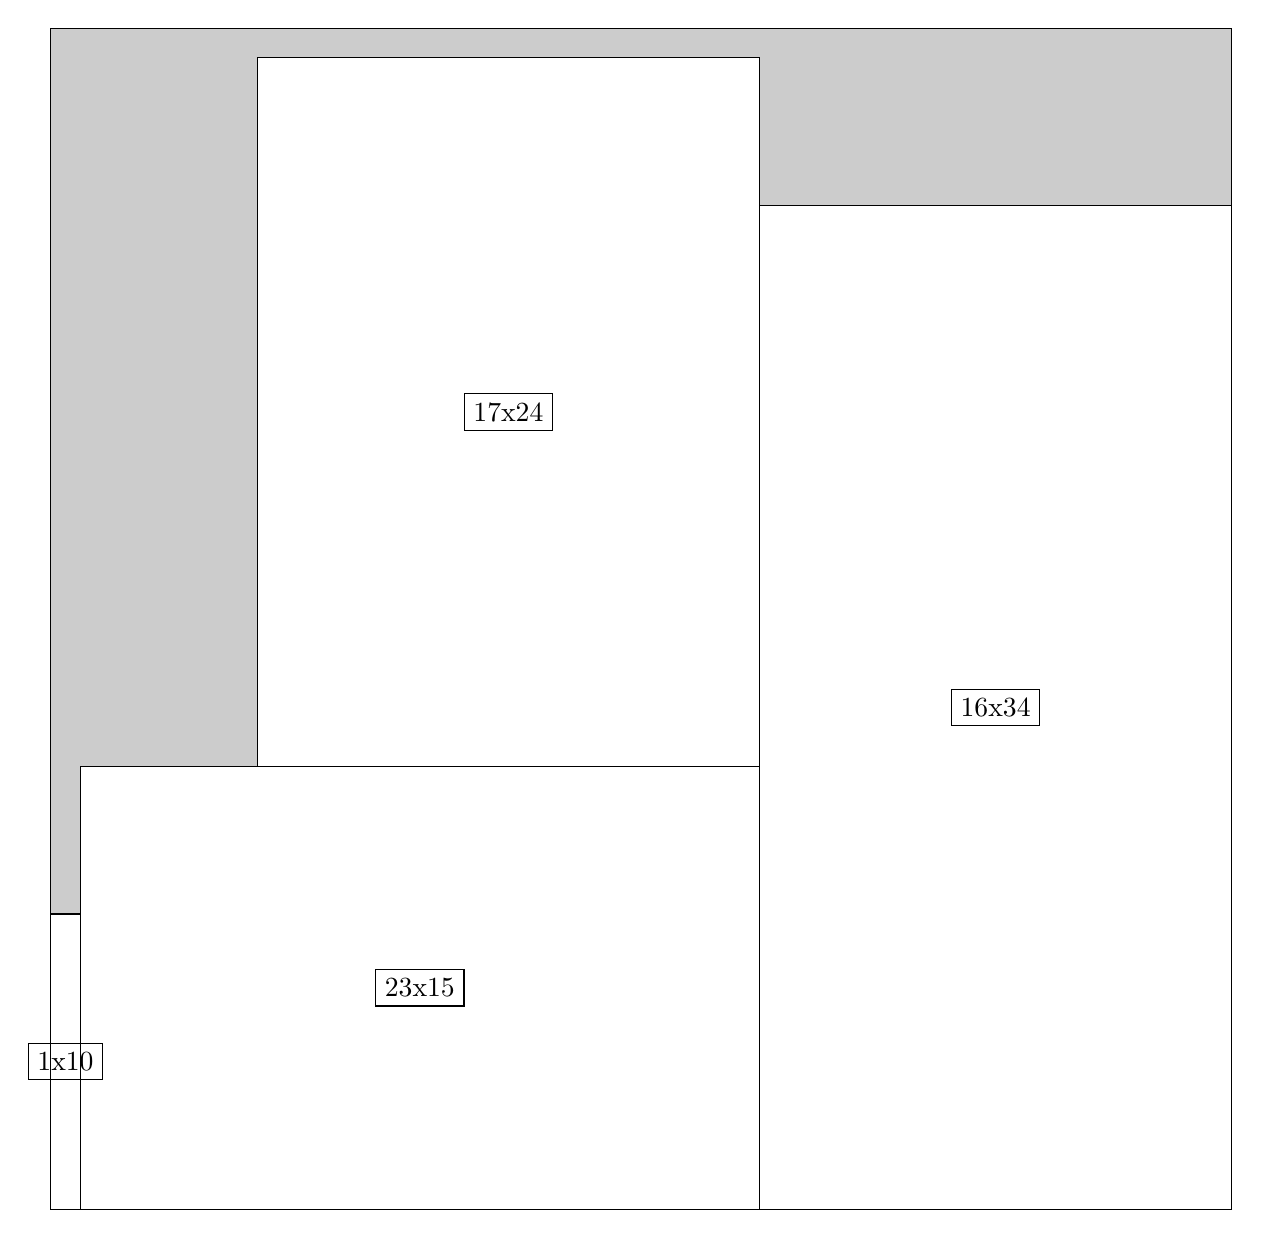
\begin{tikzpicture}[shorten >=1pt,scale=1.0,every node/.style={scale=1.0},->]
\tikzstyle{vertex}=[circle,fill=black!25,minimum size=14pt,inner sep=0pt]
\filldraw[fill=gray!40!white, draw=black] (0,0) rectangle (15.0,15.0);
\foreach \name/\x/\y/\w/\h in {16x34/9.0/0.0/6.0/12.75,23x15/0.375/0.0/8.625/5.625,1x10/0.0/0.0/0.375/3.75,17x24/2.625/5.625/6.375/9.0}
\filldraw[fill=white!40!white, draw=black] (\x,\y) rectangle node[draw] (\name) {\name} ++(\w,\h);
\end{tikzpicture}


w =16 , h =34 , x =24 , y =0 , v =544
\par
w =23 , h =15 , x =1 , y =0 , v =345
\par
w =1 , h =10 , x =0 , y =0 , v =10
\par
w =17 , h =24 , x =7 , y =15 , v =408
\par
\newpage


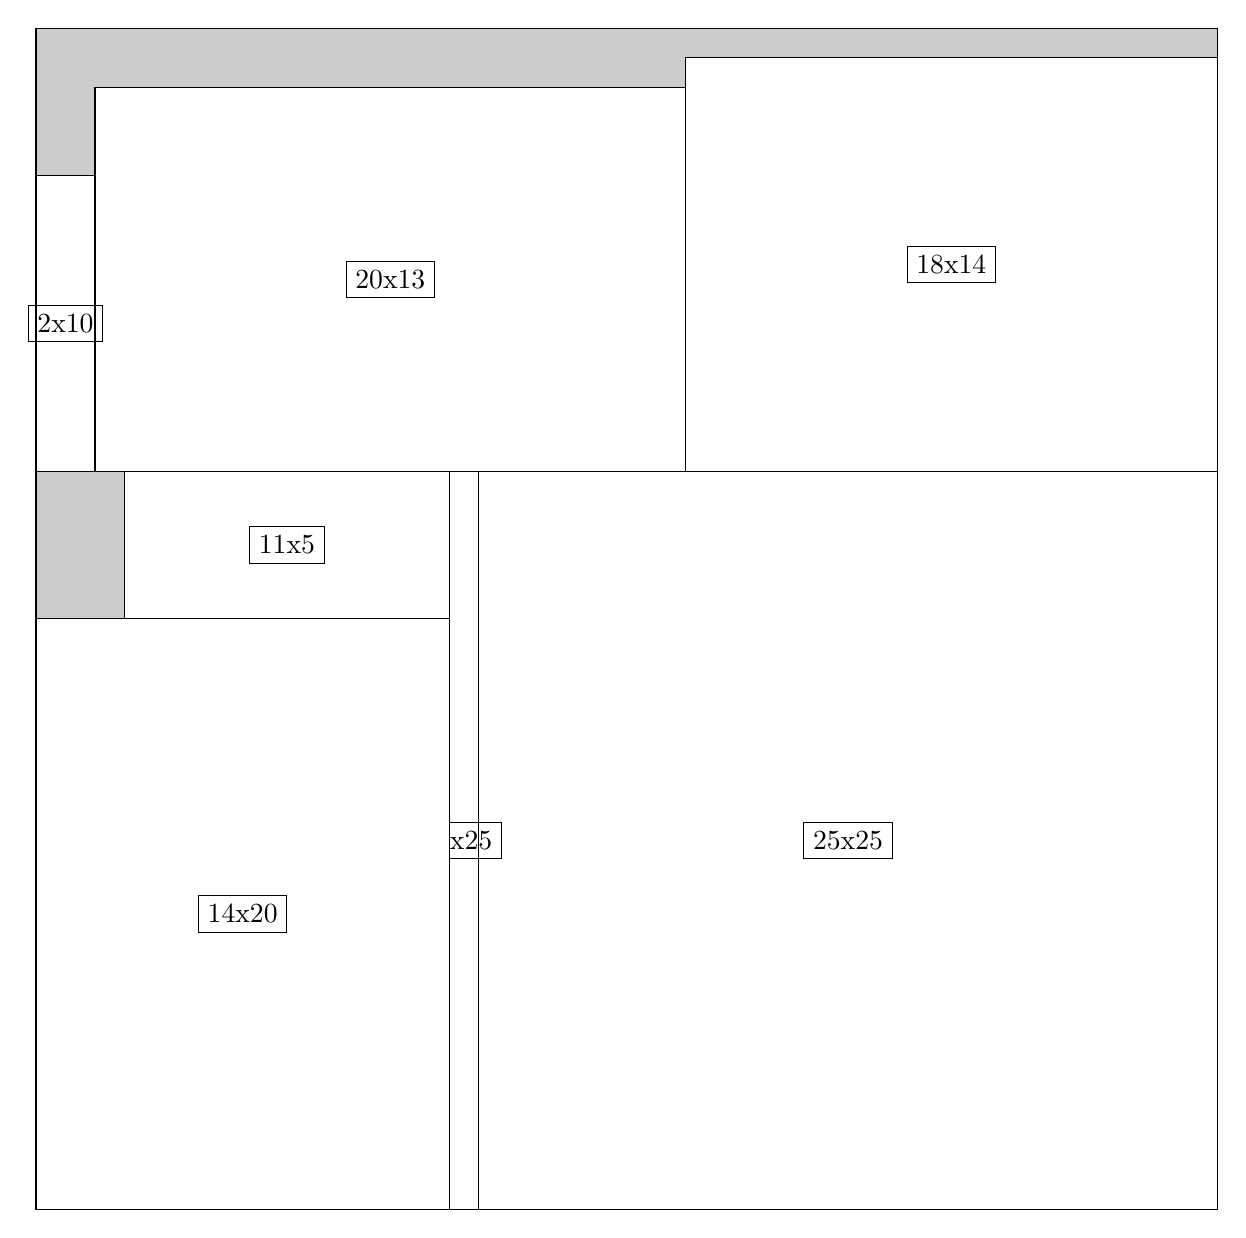
\begin{tikzpicture}[shorten >=1pt,scale=1.0,every node/.style={scale=1.0},->]
\tikzstyle{vertex}=[circle,fill=black!25,minimum size=14pt,inner sep=0pt]
\filldraw[fill=gray!40!white, draw=black] (0,0) rectangle (15.0,15.0);
\foreach \name/\x/\y/\w/\h in {25x25/5.625/0.0/9.375/9.375,1x25/5.25/0.0/0.375/9.375,14x20/0.0/0.0/5.25/7.5,11x5/1.125/7.5/4.125/1.875,18x14/8.25/9.375/6.75/5.25,20x13/0.75/9.375/7.5/4.875,2x10/0.0/9.375/0.75/3.75}
\filldraw[fill=white!40!white, draw=black] (\x,\y) rectangle node[draw] (\name) {\name} ++(\w,\h);
\end{tikzpicture}


w =25 , h =25 , x =15 , y =0 , v =625
\par
w =1 , h =25 , x =14 , y =0 , v =25
\par
w =14 , h =20 , x =0 , y =0 , v =280
\par
w =11 , h =5 , x =3 , y =20 , v =55
\par
w =18 , h =14 , x =22 , y =25 , v =252
\par
w =20 , h =13 , x =2 , y =25 , v =260
\par
w =2 , h =10 , x =0 , y =25 , v =20
\par
\newpage


\end{document}